\chapter{Числовые характеристики.}

\noindent$R = \{ Face_i \}_{i \in T}$ -- набор граней, соответствующий $\{ n_i\}_{i \in T}$.

\subsection*{\Large{Полоса набора $R$}.}

\begin{definition}[Аппроксимирующая плоскость.]
	$\Pi = \Pi(R)$ -- {\color{Black} \textbf{плоскость, аппроксимирующая вершины граней R}} в метрике 

	$$\begin{gathered}
			\rho(R, \; \Pi = \sum\limits_{i \in T}\sum\limits_{j_i}dist(v_{j_i}, \; \Pi(R)),
		\end{gathered}$$

	\noindentгде $dist(v_{j_i}, \; \Pi)$ -- евклидово расстояние от точки $v_{j_i}$ до плоскости $\Pi$, $\{ v_{j_i} \} $ -- вершины $Face_i$.

\end{definition}

\begin{remark}
	Далее, в качестве прямой, аппроксимирующей произвольный набор точек, будем использовать \textit{робастную линейную регрессию}.
\end{remark}

Развернем набор граней R на плоскости, перпендикулярной $\Pi$. 
\begin{figure}[h!]
\center{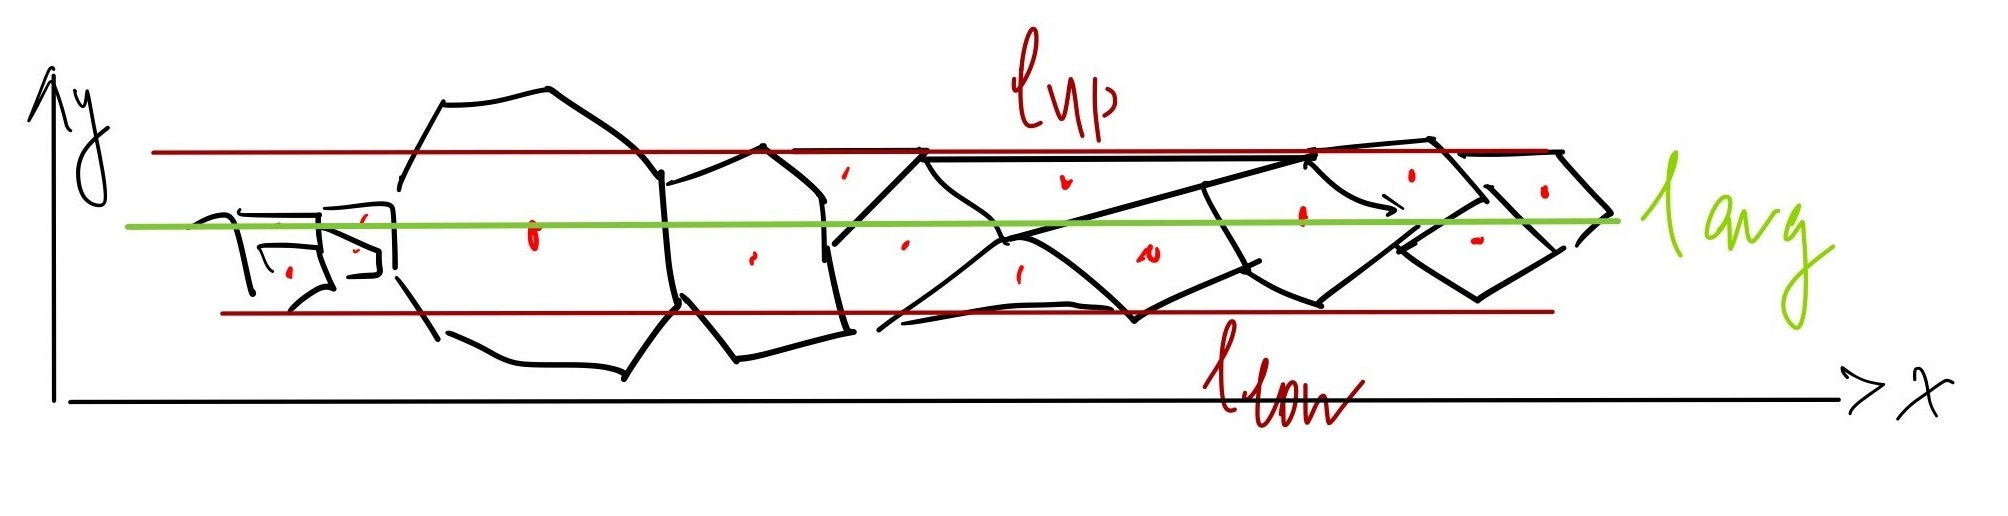
\includegraphics[scale=0.4]{Line.jpg}}
\caption{$\{ c_i\}$ -- красные точки.}
\end{figure}\newpage

Далее:
\begin{itemize}
	\item Приблизим центры граней $\{ c_i\}$ прямой $l_{avg}$.
	\item Найдем контур $Contour$ развернутого набора R.
	\item Рассмотрим вершины граней, лежащие выше прямой $l_{avg}$: $\{ v_k^{(u)}\} \in \cup_i Face_i: \; \forall \; k \; v_k^{(u)} \in Contour, \; y < v_k^{(u)}(y), \; (x, y) \in l_{avg}.$ Построим $l^{(up)}$ по набору  $\{ v_k^{(u)}\}$. Аналогично по точкам $\{ v_k^{(l)}\}$, лежащим ниже прямой $l_{avg}$, вычислим $l^{(low)}$.
\end{itemize}

\begin{definition}[Полоса рундиста ($girdle^{2D}$)]
	{\color{Black} \textbf{Полоса рундиста}} -- пространство плоскости, заключенное между $l^{(up)}$ и $l^{(low)}$ на участке $[x_{min}, x_{max}]$:
	$$\begin{gathered}
		girdle^{2D}(R):= \{ (x, y) \in \mathbb{R}^2: \; l^{(low)} \leq y \leq l^{(up)}\}.
	\end{gathered}$$
	\begin{figure}[h!]
	\center{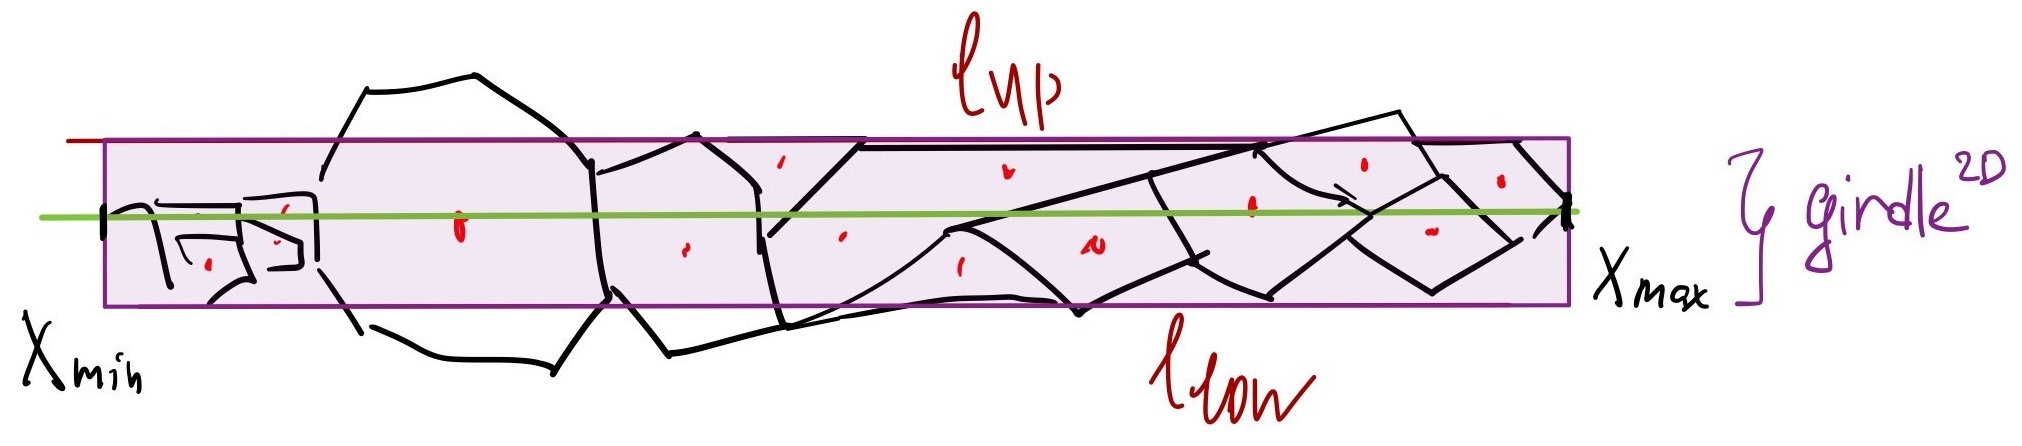
\includegraphics[scale=0.4]{Girdle.jpg}}
	\end{figure}

\end{definition}

\begin{definition}
	$x_{min} = \underset{x \in \{ v_k(x) \}}{argmin(x)}, \; x_{max} = \underset{x \in \{ v_k(x) \}}{argmax(x)}$.
\end{definition}

\begin{definition}[Размах полосы R (Amplitude).]
	$$\begin{gathered}
		Amplitude(R) := \underset{x \in [x_{min}, x_{max}]}{argmax}|l^{(up)}(x) - l^{(low)}(x)|,
	\end{gathered}$$
	где $l(x)$ -- координата $y$ точки $(x, y) \in l$.

	\begin{figure}[h!]
	\center{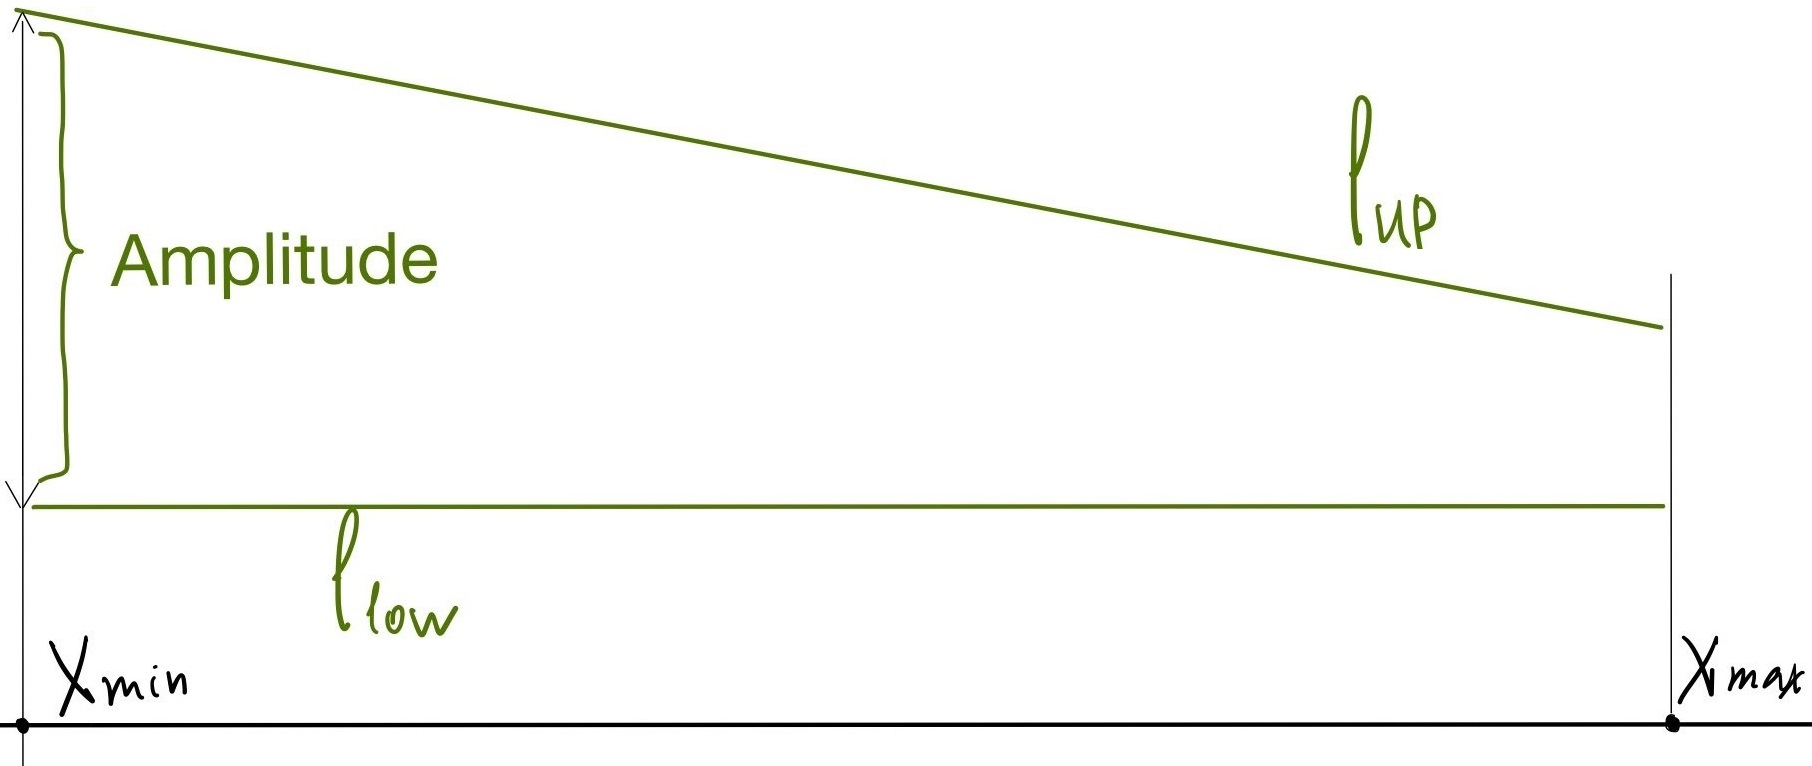
\includegraphics[scale=0.3]{Amplitude.jpg}}
	\end{figure}
\end{definition}\newpage

\begin{definition}[Параллельность $girdle^{2D}$]
	$$\begin{gathered}
		sin(R) := |sin \angle (l^{(up)}, l^{(low)})|.
	\end{gathered}$$

\end{definition}

\begin{definition}
	\noindentИзмерим, насколько сильно R выходит за свою полосу: посчитаем площадь частей граней $Face_i$, выходящих за полосу:

	$$\begin{gathered}
		S_{extern}(R) := \sum\limits_{i}Area(Face_i \cap \{ \mathbb{R}^2 \setminus girdle^{2D} \})
	\end{gathered}$$

	\begin{figure}[h!]
	\center{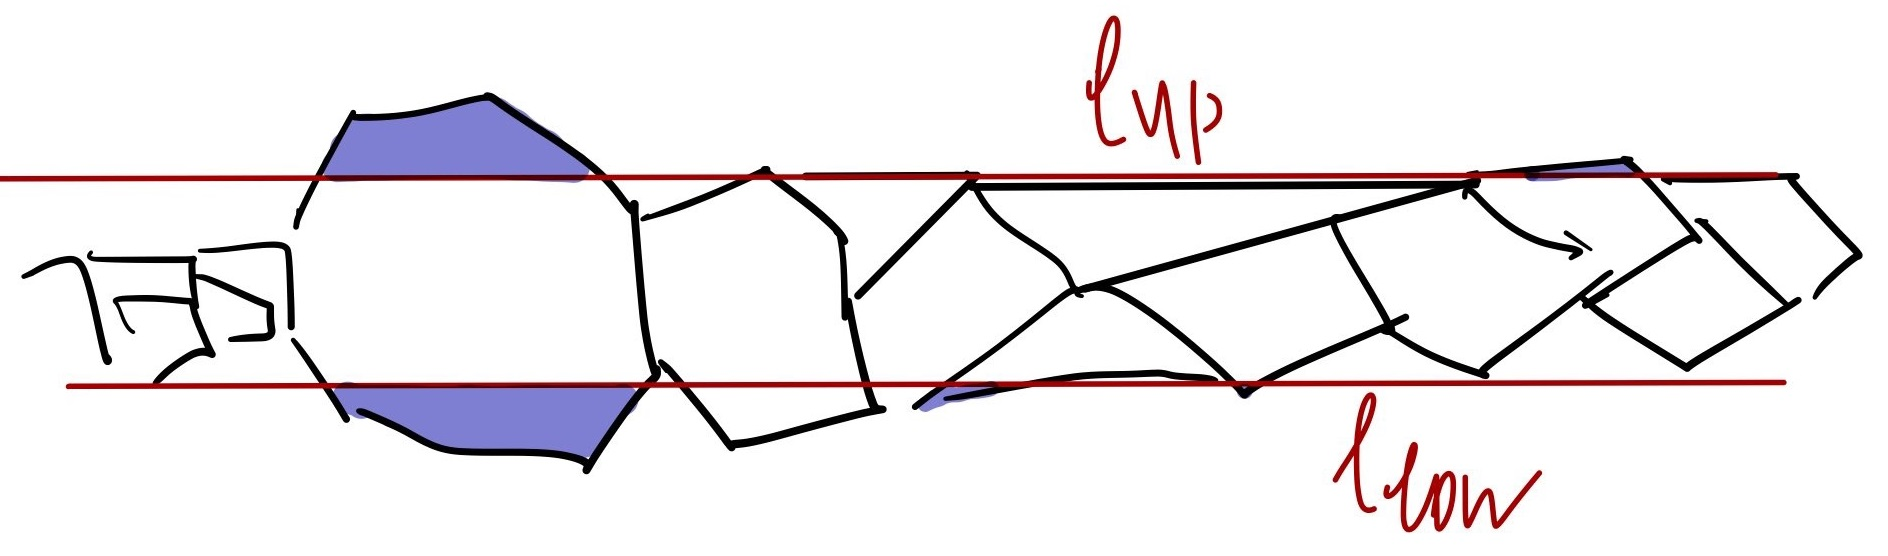
\includegraphics[scale=0.4]{Area_extern.jpg}}
	\caption{В примере на изображении выше находим суммарную площадь синих участков.}
	\end{figure}

\end{definition}

\begin{remark}
	\noindentВозможна ситуация, когда в R лежат наборы, не соответствующие (визуально) одной и той же части камня. Разобьем R на подмножества смежных граней: $R^i:\; \bigcup_i R^i = R.$ 

	\noindentОднако, может быть такое, что $\exists$ грани $\in R$, для которых среди элементов R нет смежных граней. 

	\noindentРассмотрим случай, когда такая грань $Face_{i_0}$ одна. Необходимо объединить ее с соответствующим ей набором $R^i$. Если $\exists $ вершина $v \in Face_{i_0}: \; v \in girdle^{2D}(R^i), $ то добавим $Face_{i_0}$ в $R^i$.

	\begin{figure}[h!]
	\center{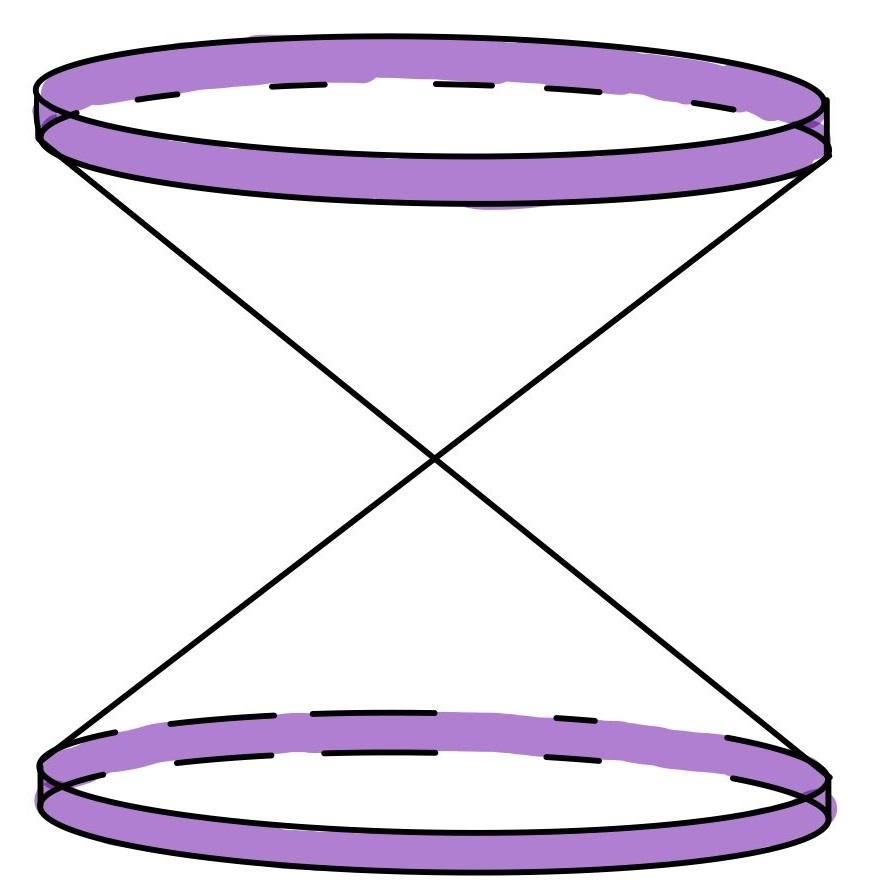
\includegraphics[scale=0.4]{TwoRund.jpg}}
	\caption{В примере на изображении выше фиолетовые части многогранника будут лежать в одном R.}
	\end{figure}\newpage
\end{remark}

\subsection*{\Large{Симметричность многогранника относительно набора $R$}.}

$\Pi$ делит $\mathbb{R}^3$ на два полупространства, $\Pi^+$ и $\Pi^-$, соответственно, делит многогранник P на $P^+ \in \Pi^+$ и $P^- \in \Pi^-$. Рассмотрим $P^+$, аналогично для $P^-$.\vspace{1cm}

\begin{figure}[h!]
\center{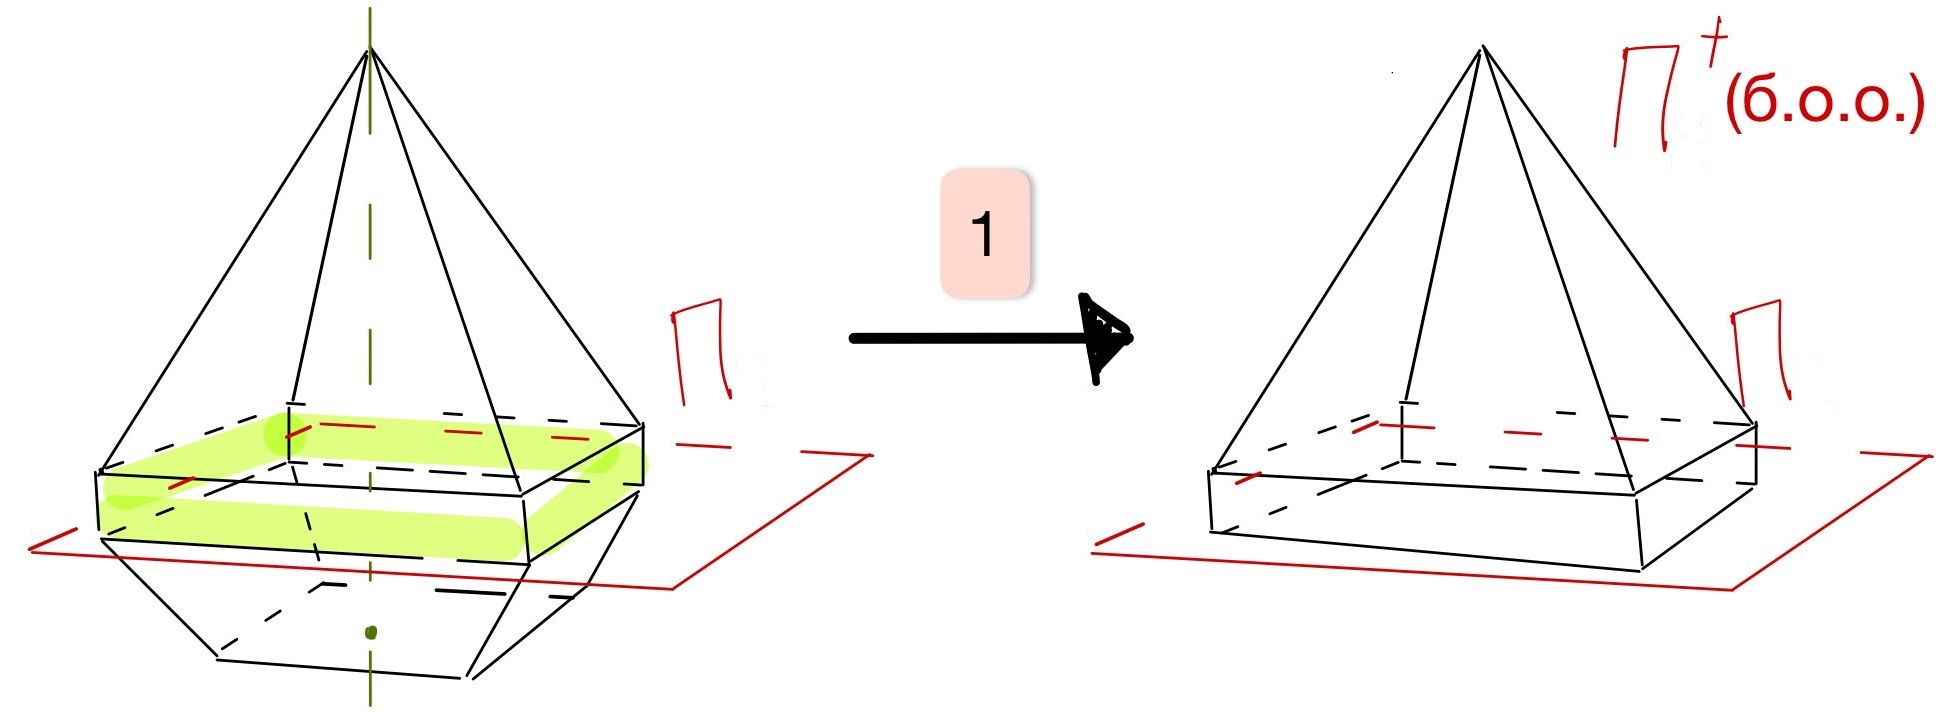
\includegraphics[scale=0.4]{PolyPlus.jpg}}
\end{figure}\vspace{1cm}

Будем пересекать $P^+$ плоскостями $\Pi_j$, параллельными $\Pi$. $CS_j(Cross Section)$ -- граница j-ого сечения, $j = 1, N_{cs}.$\newpage

\begin{figure}[h!]
\center{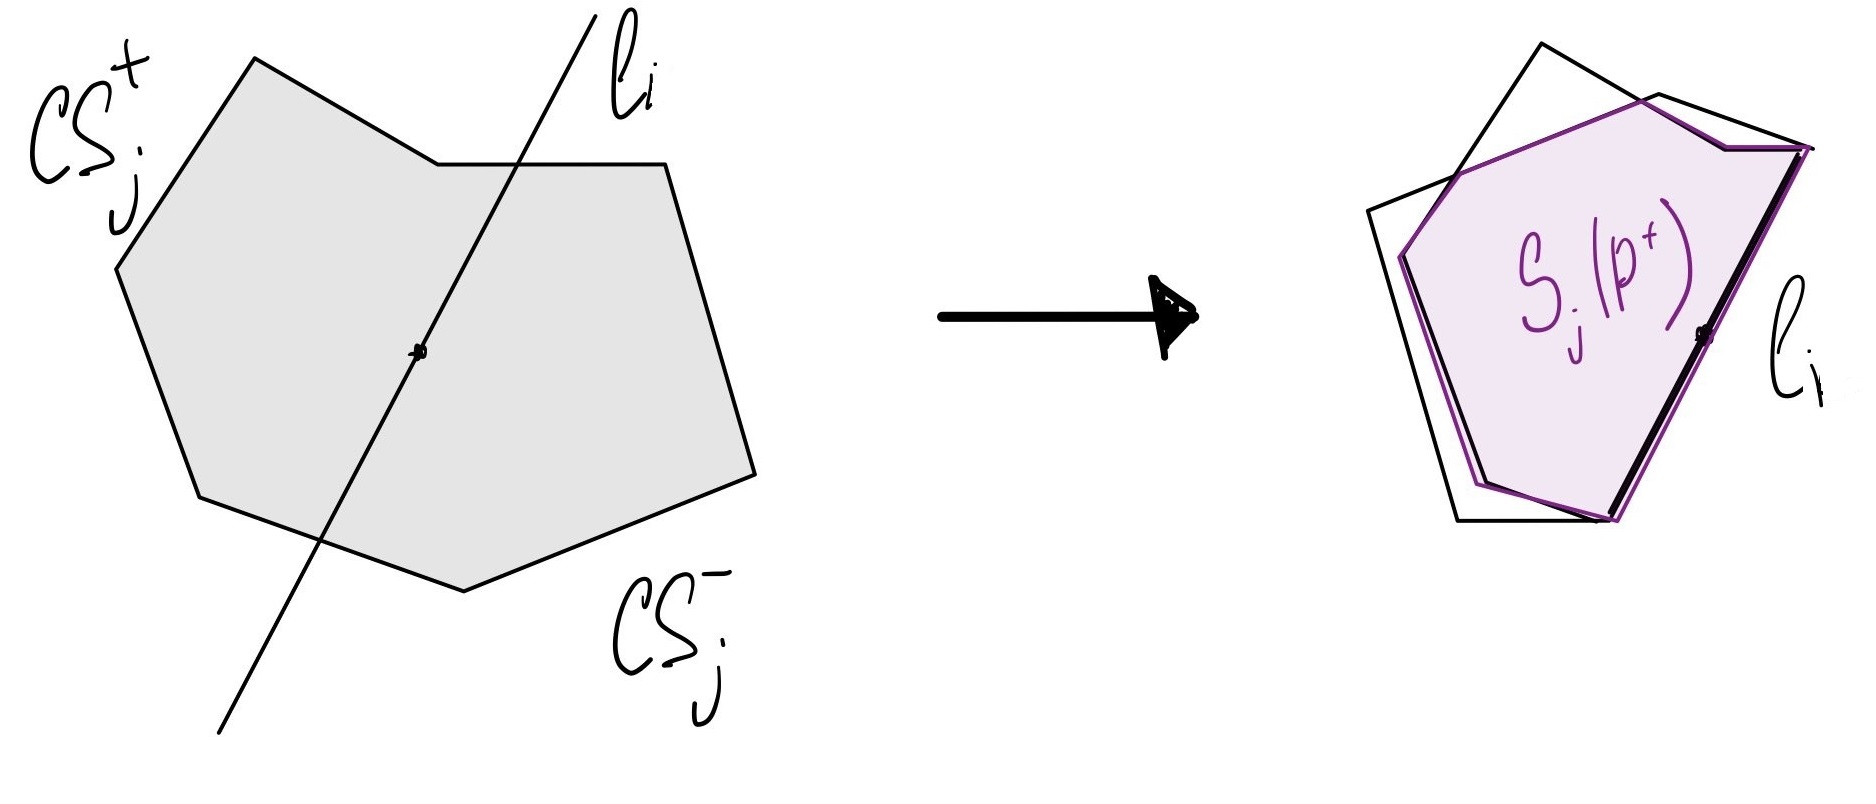
\includegraphics[scale=0.4]{Sym.jpg}}
\end{figure}

Введем меру симметричности $CS_j$. Для этого проведем $n$ прямых $l_i$ через центр многогранника P, спроецированного на $\Pi_j$, с шагом по углу $\dfrac{360}{n}$. $l_i$ делит $CS_j$ на две части: $CS_j^+, \; CS_j^-$. Отобразим $CS_j^-$ на $CS_j^+$ симметрично относительно $l_i$ (обозначение для отображенного $CS_j^-$ оставим тем же), найдем площадь пересечения и поделим ее на площадь $CS_j$ для нормировки:

$$\begin{gathered}
	S_j^i(P^+) := \dfrac{Area(CS_j^+ \cap CS_j^-)}{Area(CS_j)}.
\end{gathered}$$

Таким образом, набору R поставим в соответствие величину

$$\begin{gathered}
	Sym(R):= \sum\limits_{j = 1}^{N_{cs}}\sum\limits_{i = 1}^{n} S_j^i(P^+) + S_j^i(P^-).
\end{gathered}$$

\subsection*{\Large{Мера близости набора $R$ и аппроксимирующей ее цилиндрической поверхности Cyl.}}

R -- набор граней, Cyl -- аппроксимирующая его цилиндрическая поверхность. Для каждого множества граней R вычислим, насколько хорошо оно "ложится" на Cyl:

$$\begin{gathered}
	S_{Cyl}(R) := \dfrac{Area(R \cap Cyl)}{Area(R)}
\end{gathered}$$